\title{Music Era and Release-Market Classification}
\subtitle{DeepMIR 2026 Fall --- Homework 1}
\author{Student Name \quad (R00000000)}
\institute{Code \& checkpoints: \url{https://github.com/chijenpeng/26-fall-DeepMIR-HW1}}
\date{October 5, 2026}
\begin{document}
\maketitle
\section{Results}
\begin{frame}{Task 1: release decade 發行年代}
  \begin{columns}[T]
    \begin{column}{0.47\textwidth}
      \textbf{Best model}
      \begin{itemize}
        \item Whisper-tiny layer 1 + MERT-330M layers 5, 6, 14
        \item mean + std pooling, logistic regression
        \item 錯誤有 57\% 落在相鄰年代
      \end{itemize}
      \vspace{0.6em}
      \begin{tabular}{lcc}
        \toprule
        Model & Top-1 & Top-3 \\
        \midrule
        Hand-crafted (24-d) & .409 & .856 \\
        MERT-95M & .485 & .818 \\
        MERT-330M & .500 & \textbf{.879} \\
        \alert{+ Whisper-tiny} & \alert{\textbf{.523}} & .864 \\
        \bottomrule
      \end{tabular}
    \end{column}
    \begin{column}{0.53\textwidth}
      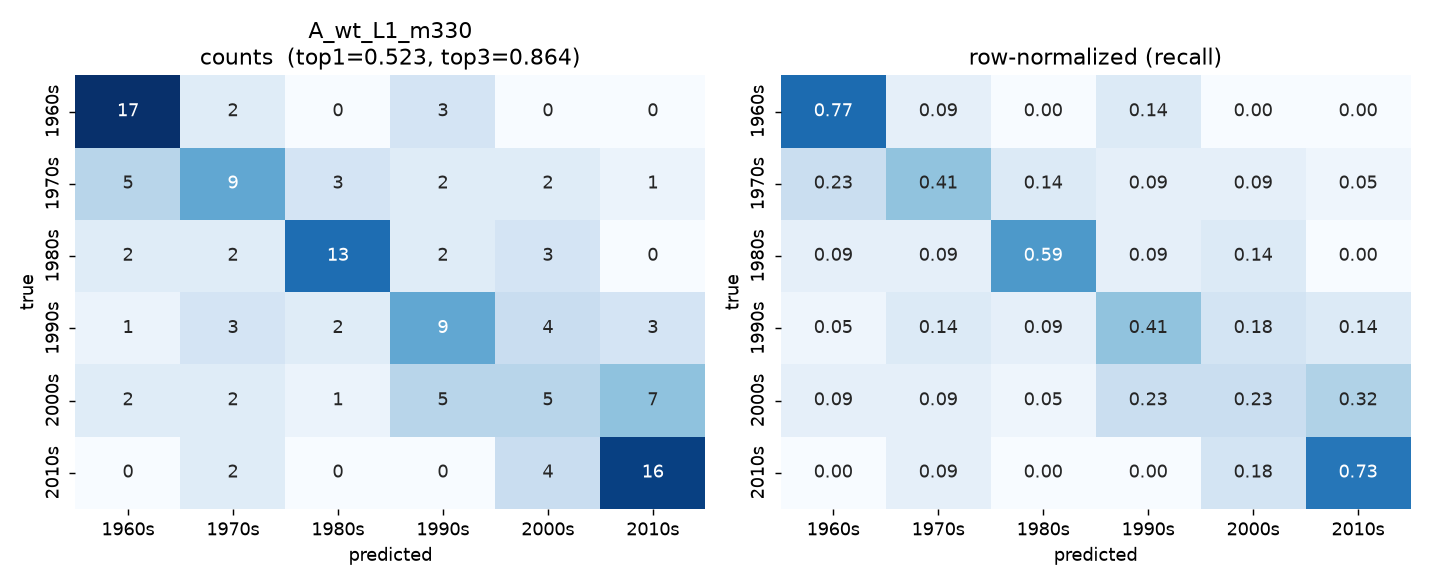
\includegraphics[width=\linewidth,trim=0 0 520 0,clip]{../../results/A_wt_L1_m330_cm.png}
    \end{column}
  \end{columns}
\end{frame}
\begin{frame}{Observation 觀察}
  \begin{itemize}
    \item Older masters have almost no sub-bass below 60 Hz; 1960s 比 2010s 少 8.6 dB。
    \item 2000s onward: brick-wall limiting, crest factor drops by 3 dB.
    \item \alert{Frozen features + linear model} beat all 14 fine-tuning runs.
  \end{itemize}
  \begin{block}{Takeaway}
    Production cues live in the shallow layers; language cues live in the deep layers.
  \end{block}
\end{frame}
\end{document}
